\begin{frame}[t]{Boltzmann Transport Equation}
        
        \begin{dmath*}
            {\frac{1}{v} \frac{\partial \psi}{\partial t} + 
                \bm \Omega \cdot \bm \nabla \psi + \Sigma_t\left(\bm 
                x,E,t\right)\psi\left(\bm x,E,\bm \Omega,t\right)} = 
                {\frac{1}{4\pi}\intop_0^{\infty} \intop_{4\pi} 
                \Sigma_s\left(\bm x,E' \rightarrow E, \bm \Omega' \rightarrow 
                \bm \Omega,t\right) \psi\left(\bm x,E',\bm \Omega',t\right) 
                d\Omega' dE'} + {\frac{\chi_p\left(\bm x,E,t\right)}{4\pi} 
                \intop_0^{\infty} \intop_{4\pi} \left(1 - \beta\left(\bm 
                x,E',t\right)\right) \nu \Sigma_f\left(\bm x,E',t\right) 
                \psi\left(\bm x,E',\bm \Omega',t\right) d\Omega' dE'} + 
                {\sum_{j=1}^{N_d} \frac{\chi_{d,j}\left(\bm x,E,t\right)}{4\pi} 
                \lambda_j C_j\left(\bm x,t\right)} + {Q\left(\bm x,E,\bm 
                \Omega,t\right)}
        \end{dmath*}
        \begin{equation*}
        \psi\left(\bm x_b, E, \bm{\Omega},t\right) = \psi^b\left(\bm x_b, E, \bm{\Omega},t\right)\ ,\quad \bm{\Omega}\cdot \bm n < 0
        \end{equation*}

\end{frame}

%%%%%%%%%%%%%%%%%%%%%%%%%%%%%%%%%%%%%%%%%%%%%%%%%%%%%%%%%%%%%%%%%%%%%%%%%%%%%%%%%

\begin{frame}[t]{Steady-State Transport Equation}
  
    \begin{dmath*}
      {\cancel{\frac{1}{v} \frac{\partial \psi}{\partial t}} + 
        \bm \Omega \cdot \bm \nabla \psi + \Sigma_t\left(\bm 
        x,E\right)\psi\left(\bm x,E,\bm \Omega\right)} = 
        {\frac{1}{4\pi}\intop_0^{\infty} \intop_{4\pi} \Sigma_s\left(\bm x,E' 
        \rightarrow E, \bm \Omega' \rightarrow \bm \Omega\right) \psi\left(\bm 
        x,E',\bm \Omega'\right) d\Omega' dE'} + {\frac{\chi_p\left(\bm 
        x,E\right)}{4\pi} \intop_0^{\infty} \intop_{4\pi} \left(1 - 
        \beta\left(\bm x,E'\right)\right) \nu \Sigma_f\left(\bm x,E'\right) 
        \psi\left(\bm x,E',\bm \Omega'\right) d\Omega' dE'} + 
        {\cancel{\sum_{j=1}^{N_d} \frac{\chi_{d,j}\left(\bm x,E\right)}{4\pi} 
        \lambda_j C_j\left(\bm x,t\right)}} + {Q\left(\bm x,E,\bm \Omega\right)}
    \end{dmath*}
    \begin{equation*}
    \psi\left(\bm x_b, E, \bm{\Omega}\right) = \psi^b\left(\bm x_b, E, 
    \bm{\Omega}\right)\ ,\quad \bm{\Omega}\cdot \bm n < 0
    \end{equation*}

\end{frame}

%%%%%%%%%%%%%%%%%%%%%%%%%%%%%%%%%%%%%%%%%%%%%%%%%%%%%%%%%%%%%%%%%%%%%%%%%%%%%%%%%

\begin{frame}[t]{Multi-Group Approximation}   
  
  \begin{figure}[h]
    \centering
    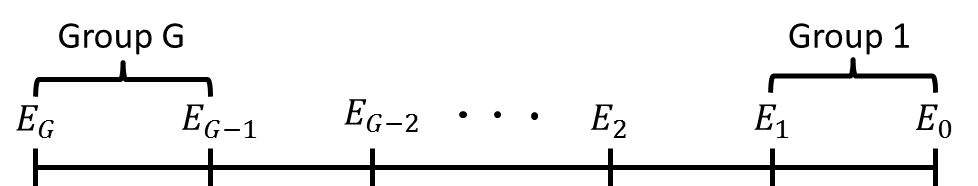
\includegraphics[width=0.8\textwidth]{MGillustration.png}
  \end{figure}
    \begin{equation*}
    \psi_g\left(\bm x, \bm \Omega\right) = \intop_{E_g}^{E_{g-1}} \psi\left(\bm 
    x, E, \bm \Omega\right) dE
    \end{equation*}
    \begin{equation*}
    \Sigma_g\left(\bm x, \bm \Omega\right) = \frac{\intop_{E_g}^{E_{g-1}} 
    \Sigma\left(\bm x, E, \bm \Omega\right) \psi\left(\bm x, E, \bm 
    \Omega\right) dE}{\intop_{E_g}^{E_{g-1}}  \psi\left(\bm x, E, \bm 
    \Omega\right) dE}
    \end{equation*}
  
 \end{frame} 
  
%%%%%%%%%%%%%%%%%%%%%%%%%%%%%%%%%%%%%%%%%%%%%%%%%%%%%%%%%%%%%%%%%%%%%%%%%%%%%%%%%
  
\begin{frame}[t]{Multi-Group Approximation}    
    
        \begin{dmath*}
            {\bm \Omega \cdot \bm \nabla \psi_g} + {\Sigma_{t,g}\left(\bm 
            x\right)\psi_g\left(\bm x,\bm \Omega\right)} = 
            {\frac{1}{4\pi}\sum_{g'=1}^G \intop_{4\pi} \Sigma_{s,g'\rightarrow 
            g}\left(\bm x,\bm \Omega' \rightarrow \bm \Omega\right) 
            \psi_{g'}\left(\bm x,\bm \Omega'\right) d\Omega'} + 
            {\frac{1}{k_{eff}}\frac{\chi_g}{4\pi} \sum_{g'=1}^{G} \intop_{4\pi} 
            \nu \Sigma_{f,g'}\left(\bm x\right) \psi_{g'}\left(\bm x,\bm 
            \Omega'\right)d\Omega' + \frac{Q_g\left(\bm x\right)}{4\pi}}
        \end{dmath*}
        \begin{equation*}\label{e:multigroupboltzmannBC}
        \psi_g\left(\bm x_b, \bm{\Omega}\right) = \intop_{E_n}^{E_{n-1}} \psi^b\left(\bm x_b, E, \bm{\Omega}\right)dE\ ,\quad \bm{\Omega}\cdot \bm n < 0
        \end{equation*}

\end{frame}

%%%%%%%%%%%%%%%%%%%%%%%%%%%%%%%%%%%%%%%%%%%%%%%%%%%%%%%%%%%%%%%%%%%%%%%%%%%%%%%%%

\begin{frame}[t]{Discrete Ordinates Approximation}
  
  \begin{itemize}
    \item Solve transport equation along fixed directions $\bm \Omega_n$
    \begin{align*}
    \bm\Omega &= \cos\left(\alpha\right)\sqrt{1-\mu_s^2}\bm i + 
    \sin\left(\alpha\right)\sqrt{1-\mu_s^2}\bm j + \mu_s\bm k \\
    \Rightarrow \bm\Omega_n &= \cos\left(\alpha_n\right)\sqrt{1-\mu_{s,n}^2}\bm 
    i + \sin\left(\alpha_n\right)\sqrt{1-\mu_{s,n}^2}\bm j + \mu_{s,n}\bm k
    \end{align*}
    \item Applies quadrature to approximate integrals
    \begin{equation*}
    \intop d\Omega = \sum_{n=1}^N w_n = 4\pi\ ,\quad \intop \bm\Omega d\Omega = 
    \sum_{n=1}^N \bm\Omega_n w_n = 0\ ,
    \end{equation*}
    \begin{equation*}
    \intop_{4\pi} f\left(\bm\Omega\right)d\Omega \approx \sum_{n=1}^N f_n w_n
    \end{equation*}
  \end{itemize}
  
\end{frame}
  
%%%%%%%%%%%%%%%%%%%%%%%%%%%%%%%%%%%%%%%%%%%%%%%%%%%%%%%%%%%%%%%%%%%%%%%%%%%%%%%%%
  
\begin{frame}[t]{Discrete Ordinates Approximation}
    
        \begin{dmath*}
            \bm\Omega_n\cdot\bm\nabla\psi_{g,n} + \Sigma_{t,g}\left(\bm x\right)\psi_{g,n}\left(\bm x\right) = {\frac{1}{4\pi}\sum_{g'=1}^G \sum_{n'=1}^N \Sigma_{g'\rightarrow g,n'\rightarrow n}\left(\bm x\right)\psi_{g',n'}\left(\bm x\right) w_{n'}} + {\frac{1}{k_{eff}}\frac{\chi_g}{4\pi} \sum_{g'=1}^G \sum_{n'=1}^N \nu\Sigma_{f,g'}\left(\bm x\right)\psi_{g',n'}\left(\bm x\right) w_{n'}} + \frac{Q_{g,n}\left(\bm x\right)}{4\pi}
        \end{dmath*}
        \begin{equation*}
        \psi_{g,n}\left(\bm x_b\right) = \psi_{g}^b\left(\bm x_b,\bm{\Omega}_n\right)\ ,\quad \bm{\Omega}_n\cdot \bm n < 0
        \end{equation*}
    
\end{frame}

%%%%%%%%%%%%%%%%%%%%%%%%%%%%%%%%%%%%%%%%%%%%%%%%%%%%%%%%%%%%%%%%%%%%%%%%%%%%%%%%%

\begin{frame}[t]{Diffusion Approximation}
    
    \begin{itemize}
      \item Assumes flux is linearly anisotropic
      \begin{equation*}
       \psi_g\left(\bm x,\bm \Omega\right) \approx 
       \frac{1}{4\pi}\left(\phi_g\left(\bm x\right) + 3\bm \Omega \cdot \bm 
       J_b\left(\bm x\right)\right)
      \end{equation*}
      \item Assumes relationship between scalar flux $\phi$ and current $J$
      \begin{equation*}
      \bm J_g\left(\bm x\right) \approx -D_g\left(\bm x\right) \bm \nabla 
      \phi_g\left(x\right)
      \end{equation*}
      \begin{equation*}
      D\left(\bm x\right)  = \frac{1}{3\left(\Sigma_{t,g}\left(\bm 
      x\right)-\sum_{g'=1}^G \Sigma_{s1,g'\rightarrow g}\left(\bm 
      x\right)\right)}
      \end{equation*}
      \item Eliminates angle dependence
      \item Simplifies streaming and scattering source terms
    \end{itemize}
  
\end{frame}

%%%%%%%%%%%%%%%%%%%%%%%%%%%%%%%%%%%%%%%%%%%%%%%%%%%%%%%%%%%%%%%%%%%%%%%%%%%%%%%%%

\begin{frame}[t]{Diffusion Approximation}
  
    \begin{dmath*}\label{e:DiffusionEquation}
        {-\bm\nabla \cdot D_g\left(\bm x\right) \bm \nabla\phi_g\left(\bm 
        x\right) + \Sigma_{t,g}\left(\bm x\right)\phi_g\left(\bm x\right) = 
        \sum_{g'=1}^G \Sigma_{s0,g'\rightarrow g}\left(\bm 
        x\right)\phi_{g'}\left(\bm x\right)} + 
        {\frac{1}{k_{eff}}\frac{\chi_g}{4\pi} \sum_{g'=1}^G 
        \nu\Sigma_{f,g'}\left(\bm x\right)\phi_{g'}\left(\bm x\right)} + 
        Q_g\left(\bm x\right)
    \end{dmath*}
    \begin{equation*}\label{e:DiffusionEquationBC}
    \frac{1}{4} \phi_g\left(\bm x_b\right) + \frac{D_g\left(\bm x_b\right)}{2} 
    \bm \cdot \bm \nabla \phi_g\left(\bm x_b\right) = J^-\left(\bm x_b\right)
    \end{equation*}
    
\end{frame}

%%%%%%%%%%%%%%%%%%%%%%%%%%%%%%%%%%%%%%%%%%%%%%%%%%%%%%%%%%%%%%%%%%%%%%%%%%%%%%%%%

\begin{frame}[t]{Scattering Approximations}
    
\begin{itemize}
    \item P$_N$ Scattering
    \begin{itemize}
      \item Uses Legendre polynomial expansion of scattering cross-section
      \item Represents scattering anisotropy using angular moments instead of 
      explicitly treating each angle
    \end{itemize}
        \begin{equation*}
        \Sigma_s\left(\bm x,\mu_s\right) = \sum_{n=0}^N \frac{2n+1}{4\pi} P_n\left(\mu_s\right) \Sigma_{sn}\left(\bm x\right)\ ,
        \end{equation*}
        \begin{equation*}
        \Sigma_{s,n}\left(\bm x\right) = 2\pi\intop_{-1}^1 \Sigma_s\left(\bm x,\mu_s\right) P_n\left(\mu_s\right) d\mu_s\ .
        \end{equation*}
      \end{itemize}
  
\end{frame}

%%%%%%%%%%%%%%%%%%%%%%%%%%%%%%%%%%%%%%%%%%%%%%%%%%%%%%%%%%%%%%%%%%%%%%%%%%%%%%%%%

\begin{frame}[t]{Scattering Approximations}
  
  \begin{itemize}
    \item Transport-Corrected P$_0$ (TCP0)
    \begin{itemize}
      \item Modifies self-scatter and total cross-sections to account for 
      anisotropy while performing isotropic calculations
      \item Neutron Leakage Conservation (NLC) Method: H-1
      \begin{equation*}
      \Sigma_{s0,g\rightarrow g} = \Sigma_{s0,g\rightarrow g} + \frac{1}{3D_g} 
      - \Sigma_{t,g}
      \end{equation*}
      \item In-Scatter Method: B-11, C-12, O-16
      \begin{equation*}
      \Sigma_{s0,g\rightarrow g} = \Sigma_{s0,g\rightarrow g} - 
      \frac{1}{\phi_{1,g}}\sum_{g'=1}^G \Sigma_{s1,g'\rightarrow g}\phi_{1,g'}
      \end{equation*}
      \item Out-Scatter Method: All other isotopes
      \begin{equation*}
      \Sigma_{s0,g\rightarrow g} = \Sigma_{s0,g\rightarrow g} - \sum_{g'=1}^G 
      \Sigma_{s1,g\rightarrow g'}
      \end{equation*}
    \end{itemize}
\end{itemize}

\end{frame}